\documentclass[twoside,french]{article}
\usepackage[francais]{babel}
\usepackage[T1]{fontenc}
\usepackage[utf8]{inputenc}
\usepackage[letterpaper]{geometry}
\usepackage{amsmath}
\usepackage{graphicx}

% For source code coloring and formatting
\usepackage{listings} 
\lstset{mathescape,basicstyle=\ttfamily}% Allow escaping to LaTeX inside $..$

\usepackage[pdftex,
      pdfauthor={Guillaume Legrain & Florian Martin},
      pdftitle={Projet Java A3P},
      colorlinks
      ]{hyperref}

\setlength{\topmargin}{-0.5in}
\setlength{\textheight}{9in}
\setlength{\oddsidemargin}{.125in}
\setlength{\textwidth}{6.25in}


\begin{document}

% \begin{titlepage}

\title{Projet Java A3P}
\date{\today}
\author{Guillaume Legrain \\
        Florian Martin \\
        E3S}
\maketitle
\begin{abstract}
Pac-Man dans un nouveau monde, sous un nouvel angle.\vspace{-2ex}
\end{abstract}
% \end{titlepage}

\section{Présentation du projet}
Vous êtes Pac-Man, perdu dans un étrange labyrinthe peuplé de fantômes. Vous voulez vous échapper.
Mais il faut trouver la clef de la sortie ainsi que des fruits pour affronter les fantômes qui en
bloquent l’accès.

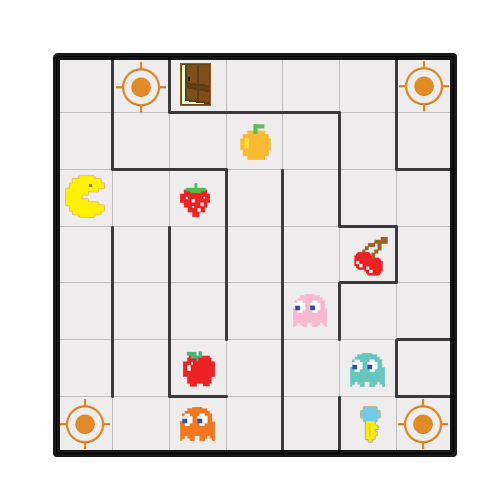
\includegraphics[scale=0.8]{graphics/Plan-Projet-1.png}

\section{Buts}
   \begin{itemize}
      \item But principal: trouver la clef pour pouvoir ouvrir la porte et sortir du labyrinthe.
      \item Les fantômes sont dangereux ! Il faut donc trouver et manger assez de fruits pour
      pouvoir les affronter.
      \item Pour aller plus vite, Pac-Man peut utiliser des téléporteurs. Mais attention, ils ne 
      sont pas toujours très fiable et peuvent parfois conduire à des pièces sans issues.
   \end{itemize}

\section{Idées ...}
Note: Tous ces points ne seront pas forcément implémentés vu que nous ne pouvons pas encore 
vraiment savoir ce qui est envisageable à notre niveau.
   \begin{itemize}
      \item Chaque case du labyrinthe sera en fait une "pièce" avec des sorties
      (Nord, Sud, Est, West)
      \item Le joueur pourra choisir parmi plusieurs labyrinthes ( peut être même en 
      créer lui-même, dans un fichier que le jeu va "parser" avant de démarrer). %Une première approche
      %sera d'essayer de charger le niveau enregistré au format JSON ou XML et de le parser. %avec 
      %\href{https://github.com/douglascrockford/JSON-java}{JSON-java} ou \href{https://code.google.com/p/google-gson/}{google-gson}
      %par exemple.
      \item EN PLUS de la console (avec le "prompt"), le joueur pourra se déplacer avec les 
      touches du clavier (Up, down, left, right).
      \item Le Pac-Man se déplace aussi, en temps réel sur l'écran.
      \item Dessiner le plan du labyrinthe en Java (ou autre si mieux ...) suivant sa description
      plutôt que d'afficher une ou des images statiques.
      \item Créer une carte évolutive qui se met a jour lors du passage dans une piece.
      \item Imposer un certain nombre de fruit pour vaincre un type de fantôme.
      \item Insérer une musique dans le jeu.
      \item Insérer des sons lors de la récupération d'objet (clé, fruit) ou l'appartion d'un fantôme
   \end{itemize}

\section{Organisation d'un plan}
   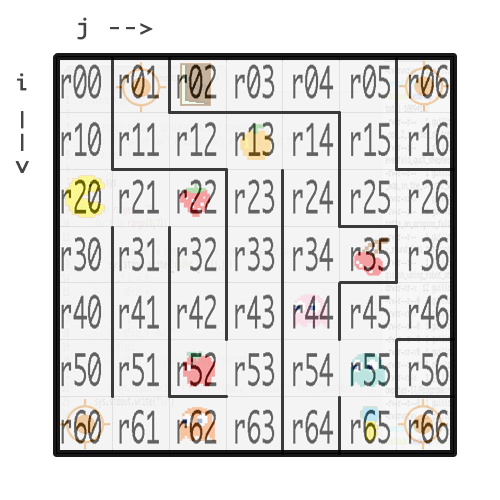
\includegraphics[scale=0.4]{graphics/Plan-Projet-1_numbered.png} \\
   Chaque "Room" est représentée par rij indiquant sa position sur le plan.
   Chaque "Room" possède des attributs indiquant la position de la case suivante ou un mur (avec un \lstinline|null| )


\end{document}
